\documentclass{bioinfo}
\copyrightyear{2015} \pubyear{2015}
\usepackage{url}
\usepackage{booktabs}
\usepackage[table]{xcolor}
\usepackage{float}
\newcommand{\myColor}{black}
\newcommand{\mySecondColor}{red}
\access{Advance Access Publication Date: Day Month Year}
\appnotes{Manuscript Category}

\begin{document}
\firstpage{1}
\subtitle{Sequence analysis}

\title[Protein interaction sites prediction]{DELPHI: accurate deep ensemble model for protein interaction sites prediction}
\author[Y.Li et al.]{Yiwei Li\,$^1$, 
\textcolor{\mySecondColor}{G.~Brian Golding\,$^2$}
 and Lucian Ilie\,$^{1,*}$}
\address{$^1$Department of Computer Science, The University of Western Ontario London, ON, N6A 5B7, Canada \textcolor{\mySecondColor}{and $^2$Department of Biology, McMaster University, Hamilton, Ontario, Canada
L8S 4K1}}

\corresp{$^\ast$To whom correspondence should be addressed: \texttt{ilie@uwo.ca}}

\history{Received on XXXXX; revised on XXXXX; accepted on XXXXX}

\editor{Associate Editor: XXXXXXX}

\abstract{\textbf{Motivation:} Proteins usually perform their functions by interacting with other proteins, which is why accurately predicting protein-protein interaction (PPI) binding sites is a fundamental problem. Experimental methods are slow and expensive. Therefore, great efforts are being made towards increasing the performance of computational methods.\\
\textbf{Results:} We propose DELPHI (DEep Learning Prediction of Highly probable protein Interaction sites), a new sequence-based deep learning suite for PPI binding sites prediction. DELPHI has an ensemble structure which combines a CNN and a RNN component with fine tuning technique. Three novel features, HSP, position information, and ProtVec are used in addition to nine existing ones. \textcolor{\myColor}{We comprehensively compare DELPHI to nine state-of-the-art programs on five datasets, and DELPHI outperforms the competing methods in all metrics even though its training dataset shares the least similarities with the testing datasets. In the most important metrics, AUPRC and MCC, it surpasses the second best programs by as much as 18.5\% and 27.7\%, resp. We also demonstrated that the improvement is essentially due to using the ensemble model and, especially, the three new features.} \\
\textbf{Availability:} \textcolor{\mySecondColor}{ The DELPHI web server, datasets, and results of in this study are freely available at\\ \texttt{www.csd.uwo.ca/\textasciitilde{}yli922/index.php}.\\
The trained models, the DELPHI standalone source code, and the feature computation pipeline are freely available at \texttt{github.com/lucian-ilie/DELPHI}.} \\
\textbf{Contact:} \href{ilie@uwo.ca}{ilie@uwo.ca}\\
\textbf{Supplementary information:} Supplementary data are available at \textit{Bioinformatics}
online.}
\maketitle

\section{Introduction}
Protein-protein interactions (PPI) play a key role in many cellular processes such as signal transduction, transport and metabolism \citep{zhang2018review}. Proteins interact by forming chemical bonds with other proteins. The bonding amino acid residues are protein-protein interaction binding sites. Detecting PPI binding sites helps understand cell regulatory mechanisms, locating drug target, predicting protein functions \citep{bonetta2010interactome}. Databases like PDB \citep{berman2002protein} store protein binding sites information deriving from the 3D structure of each protein, but the available protein structures are limited. Experimental methods such as two-hybrid assay and affinity systems are usually time and labour intensive \citep{shoemaker2007deciphering}. Computational methods are needed to bridge the gap, and many have been developed \citep{cao2006enhanced, ofran2007isis, du2009improved, chen2009sequence, london2010structural, chen2010sequence, murakami2010applying, xue2011homppi, amos2011binding, jones2012psicov, asadabadi2013predictions, singh2014springs, wang2014fast, geng2015prediction, laine2015local, hwang2016hybrid, maheshwari2015prediction, liu2016prediction, wei2016protein, maheshwari2016template, jia2016ippbs, zhang2019sequence, wang2019protein, zhang2019scriber, zeng2019protein, xie2020prediction}. Out of the above mentioned twenty six computational methods, all but one are machine learning based. Computational methods can be classified into three categories, sequenced based, structure based, and combined. Among them, sequence-based approaches are usually faster  and cheaper, and have the advantage that sequence information, unlike structure, is much more readily available.

Machine learning methods use feature groups to represent each protein sequence. Widely used features such as position-specific scoring matrix (PSSM), evolutionary conservation (ECO), putative relative solvent accessibility (RSA) have been assessed in \citep{zhang2019comprehensive}. High-scoring segment pair (HSP) has been used in previous methods for PPI prediction \citep{li2017sprint}. One-hot vectors \citep{zhang2019sequence, zeng2019protein} and amino acid embedding \citep{asgari2015continuous, heinzinger2019modeling, asgari2019probabilistic} have also been empirically explored to represent protein sequences.

The learning structure is crucial to PPI binding sites classification problems. Previously explored architectures include random forest \citep{wei2016protein, wang2019protein}, SVM \citep{wei2016protein}, logistic regression \citep{zhang2019scriber}, Bayes classifier \citep{murakami2010applying}, artificial neural networks \citep{singh2014springs}. Recently, convolutional neural network (CNN) \citep{zeng2019protein} and recurrent neural network (RNN) \citep{zhang2019sequence} have also been applied to solve this problem. 

We introduce a new sequence-based PPI binding sites prediction method, DELPHI (DEep Learning Prediction of Highly probable protein Interaction sites), that combines a CNN and a RNN structure with fine tuning technique. It uses twelve feature groups to represent protein sequences including three novel features, high-scoring segment pair (HSP), position information, and a reduced 3-mer amino acid embedding (ProtVec1D). We have comprehensively compared DELPHI with nine state-of-the-art programs on five datasets. DELPHI provides the best predictions in all metrics. 

The contributions of the DELPHI study are as follows. \textcolor{\myColor}{
First, a novel fine tuned ensemble model combing CNN and RNN is constructed. Second, three novel features, which are believed to be used the first time in PPI binding site prediction, are introduced. Third, a data processing and feature construction suite, is provided, aiming to alleviating the difficulty of tedious feature computation by the users.}

\begin{methods}
\section{Materials and Methods}
\subsection{Datasets}
\textcolor{\myColor}{Following the modern machine applications development process, we use three sets of data to train and evaluate the performance of DELPHI: training, validation, and testing. The model is trained on the training data and validated on the validation data to ensure low variance i.e. avoid overfitting. After several iterations of tuning, the model is obtained and ran on the independent testing data, and then performance on testing data is reported. Note that the model never observes the testing data during the training and validation process.}

\subsubsection{Testing datasets}\label{testing_data}
\textcolor{\myColor}{In order to be able to test on common benchmark data, we choose first the testing datasets, then construct the training datasets such that they are highly dissimilar with testing.}

\textcolor{\myColor}{Five datasets are used in the comparative assessment. We name them by the size of the data: Dset\_186, Dset\_72, Dset\_164, Dset\_448, and Dset\_355. The first four are publicly available datasets from previous studies \citep{murakami2010applying} \citep{dhole2014sequence} \citep{zhang2019scriber}, and the last one, Dset\_355, is a subset of Dset\_448. Dset\_186, Dset\_72, Dset\_164 have been widely used and explored as benchmark datasets by numerous publications; Dset\_448 is more recent.} 

\textcolor{\myColor}{
Dset\_186 and Dset\_72 were constructed by \cite{murakami2010applying}. Dset\_186 was built based on a PDB collection \citep{berman2002protein}, to which a six-step filtering process was applied to refine the data including removing structures with missing residues, removing chains with the same UniprotKB/Swiss-Prot accession, removing transmembrane proteins, removing dimeric structures, removing proteins with buried surface accessibility and interface polarity under certain range, and similarities elimination. Dset\_72 was constructed based on the protein-protein benchmark set version 3.0 \citep{hwang2008protein} with the similarities with Dset\_186 removed.
}

\textcolor{\myColor}{
Dset\_164 was constructed by \cite{dhole2014sequence} with the same filtering technique as for Dset\_186 and Dset\_72 on newly annotated proteins in PDB since the publication of Dset\_186 (Jun.~2010 to Nov.~2013). 
}

\textcolor{\myColor}{
Dset\_448 was constructed by \cite{zhang2019scriber}. The raw data of Dset\_448 was from the BioLip database \citep{yang2012biolip} where binding sites are defined if the distance between an atom of a residues and an atom of a given protein partner <0.5 \AA{} plus the sum of the Van der Waals radii of the two atoms. The raw data was further processed by removing protein fragments, mapping BioLip sequences to UniProt sequences, and clustering so that no similarities above 25\% are shared within Dset\_448. This dataset is the most recent one as well as the largest. }
\textcolor{\myColor}{
Dest\_448 cannot be used to test one of the top competing programs, DLPred, because it contains 93 proteins that share more than 40\% similarity with DLPred's training set. We built Dset\_355 by removing these proteins from Dset\_448.}

\textcolor{\myColor}{
Details of the size and the number of binding residues are given in Table \ref{tab_dataset}. With the exception of Dset\_355, the datasets are nearly disjoint; see Table~S1 in the Supplementary material.}
%According to the PSI-CD-HIT results, the training datasets of DLPred and SCRIBER still contain some proteins that share more than 25\% similarity to Dset\_186,  Dset\_72, and Dset\_164. However, we kept these testing datasets untouched because otherwise we would have to remove too many proteins from them. The training datasets of the competing programs can not be changed because the models are pre-trained. Note that all testing data share less than 25\% similarity to the training dataset of DELPHI. 

\subsubsection{Training and validation datasets}
\textcolor{\myColor}{
We construct next our training and validation data such that there are no similarities above 25\% between (i) training and validation data and (ii) between testing and the union of training and validation. Also, we want relatively large training data as it is beneficial for deep learning models.}

\textcolor{\myColor}{
We first obtained a large, high quality dataset from a recent survey paper \citep{zhang2019comprehensive}. In this dataset, Uniprot sequences are annotated with Protein, DNA, RNA, and small ligands binding information at the residue level. We further processed this dataset as follows. First, we kept only the sequences with protein-protein binding information to focus on protein-protein binding. Then we removed any sequences from training dataset sharing similarities above 25\%, as measured by PSI-CD-hit \citep{li2006cd,fu2012cd}, with any sequences in the five testing datasets. It is well acknowledged that similar sequences between training and testing datasets negatively affect the generalization of the evaluated performance of a machine learning model. Also, proteins with higher levels of similarity can be accurately predicted by the alignment-based methods \citep{zhang2018review}. The similarity threshold is picked differently by different programs ranging from 25\% to 50\%. We picked the strictest value of 25\% to match to one of the closest competing programs, SCRIBER \citep{zhang2019scriber}, for a fair comparison. We used PSI-CD-HIT because it is fast, accurate and well maintained in the CD-HIT suite. Also, it is able to cluster sequences with similarity at low as 25\%, whereas CD-HIT works only down to 40\%. Finally, we ran PSI-CD-hit again on the rest of the protein sequences so no sequences shared more than 25\% similarities. This ensures the training data is as diverse as possible as well as the dissimilarity between the training and validation dataset. A dataset of 9,982 protein sequences was constructed. From it, we randomly pick eight ninth (8,872) as the training dataset and one ninth (1,110) as the validation dataset. }

\subsection{Input features}
DELPHI uses 12 features groups, shown in Table \ref{tab_feature}, which gives also the dimension and each. Thus, each input is represented by a 39 dimensional feature vector profile. To the best of our knowledge, this study is the first time that HSP, ProtVec1D, and position information are being used in binding sites classification problems. The computation of each of these two new features is described next.

\begin{table}[H]
    \centering
    \caption{The datasets used for training, validation, and testing. The columns give, in order, the dataset names, the number of proteins in each dataset, the total number of residues, the number of binding, and the number of non-binding residues in each dataset, and the percentage of the binding residues out of total.}
    \begin{tabular}{@{}l*{5}{r}@{}}
    \toprule
    Dataset & Proteins & \multicolumn{3}{c}{Residues} & \multicolumn{1}{c@{}}{binding} \\ \cline{3-5}
    & & total & binding & non-binding & \multicolumn{1}{c@{}}{\% of total}\\ \hline
    Dset\_448 & 448   & 116,500 & 15,810 & 100,690 & 13.57 \\
    Dset\_355 & 355   & 95,940 & 11,467 & 84,473 & 11.95 \\
    Dset\_186 & 186   & 36,219 & 5,517 & 30,702 & 15.23 \\
    Dset\_72 & 72    & 18,140 & 1,923 & 16,217 & 10.60 \\
    Dset\_164 & 164   & 33,681 & 6,096 & 27,585 & 18.10 \\
    Train+Validate & 9,982 & 4,254,198 & 427,687 & 3,826,511 & 10.05 \\
    \hline
    \end{tabular}%
    \label{tab_dataset}%
\end{table}%

\begin{table}[H]
  \centering
  \caption{The feature groups used by DELPHI. The first column indicates the name of each feature. The second column describes the program used to obtain the feature. ``Load'' means the value for a specific amino acid is known from previous work, and it is loaded in the DELPHI program. ``Compute'' means DELPHI performs additional computation to that feature. The last column shows the dimension of each feature group. Full details are given in the text.}
    \begin{tabular}{@{}ll@{}r@{}}
    \toprule
    Feature & Program & Dimension \\
    \midrule
    High-scoring segment pair (HSP) & Compute & 1 \\
    3-mer amino acid embedding (ProtVec1D) & Load/compute & 1 \\
    Position information & Compute & 1 \\
    Position-specific scoring matrix (PSSM) & Psi-Blast & 20 \\
    Evolutionary conservation (ECO) & Hhblits & 1 \\
    Putative relative solvent accessibility (RSA) & ASAquick & 1 \\
    Relative amino acid propensity (RAA) & Load  & 1 \\
    Putative protein-binding disorder & ANCHOR & 1 \\
    Hydropathy index & Load  & 1 \\
    Physicochemical characteristics & Load  & 3 \\
    Physical properties & Load  & 7 \\
    PKx   & Load  & 1 \\
    \bottomrule
    \end{tabular}%
  \label{tab_feature}%
\end{table}%

High-scoring segment pair (HSP): An HSP is a pair of similar sub-sequences between two proteins. The similarities between two sub-sequence of the same length are measured by scoring matrices such as PAM and BLOSUM. SPRINT \citep{li2017sprint} is used for computing all HSPs as it detects similarities fast and accurately among all proteins in training and testing. After obtaining the HSPs, the score for the $i$th residue, $P[i]$, of a testing protein $P$, denoted $\text{HSP}_{\text{score}}(P[i])$, is calculated as follows. Assume we have an HSP, $(u,v)$, between $P$ and a training protein $Q$ such that $u$ covers the residue $P[i]$, that is, position $i$ in $P$ is within the range covered by $u$. Let $j$ be the position in $Q$ that corresponds to $i$, that is, the distance in $P$ from the beginning of $u$ to $i$ is the same as the distance in $Q$ from the beginning of $v$ to $j$. If $Q[j]$ is a known interacting residue, then we add the PAM120 score between $P[i]$ and $Q[j]$ to the HSP score of $P[i]$:
\[
\text{HSP}_{\text{score}}(P[i]) = \!\!\!\!\!\!\sum_{\stackrel{\text{\tiny HSPs covering $P[i]$}}{\text{\tiny $Q[j]$ interacting residue}}}\!\!\!\!\!\! \max(0, \text{PAM120}(P[i], Q[j])) \ .
\]
The 3-mer amino acid embedding (ProtVec1D): We developed this feature based on ProtVec \citep{asgari2015continuous}. ProtVec uses word2vec \citep{mikolov2013distributed} to construct a one hundred dimensional embedding for each amino acid 3-mer. It is shown in \citep{asgari2015continuous} that ProtVec can be applied to problems such as protein family classification, protein visualization, structure prediction, disordered protein identification, and protein-protein interaction prediction. Since using the ProtVec embedding in our program slows down significantly the deep learning model, especially during training, we replaced the one hundred dimensional vector by one dimensional value, which is the sum of the one hundred components; we call this ProtVec1D. According to our tests, ProtVec1D achieves, in connection with the other features, the same prediction performance as ProtVec.

Position information: In natural language processing tasks, position information is shown useful. The popular network Bert \citep{devlin2018bert} utilizes this information to guide its translation process. It is also shown by DeepPPISP \citep{zeng2019protein} that the global information of a protein helps the prediction of interfaces. Inspired by the two networks, we use the position information of each amino acid as an input feature, as it provides global information. The position of an amino acid in a protein is in the range of 1 to the length of the protein. Then the position is divided by protein's length so that the value is between 0 to 1.

Position-specific scoring matrix (PSSM): PSSM matrices are widely used in protein interaction related problems. They contain the evolutionary conservation of each amino acid position by aligning an input sequence with protein databases. The PSSM matrices are computed using PSI-Blast \citep{altschul1997gapped} with the expectation value (E-value) set to 0.001 and the number of iterations set to 3. PSI-Blast performs multiple alignment on each input sequence against the non-redundant database. 

Evolutionary conservation (ECO): ECO also contains evolutionary conservation, but in a more compact way. To compute the ECO score, the faster multiple alignment tool HHBlits \citep{remmert2012hhblits} is run against the non-redundant Uniprot20 database with default parameters. The one dimensional conservation value is computed using the formula described in \citep{zhang2019comprehensive}.

Putative relative solvent accessibility (RSA): The solvent accessibility is predicted using ASAquick \citep{faraggi2014accurate}. The values are obtained in the from rasaq.pred file in each output directory.

Relative amino acid propensity (RAA): The AA propensity for binding is quantified as relative difference in abundance of a given amino acid type between binding residues and the corresponding non-binding residues located on the protein surface. The RAA for each amino acid type is computed by \cite{zhang2019comprehensive} using the program of  \cite{vacic2007composition}.

Putative protein-binding disorder: The putative protein-binding disorder is computed using the ANCHOR program \citep{dosztanyi2009anchor}.

Hydropathy index: Hydrophobicity scales is experimentally determined transfer free energies for each amino acid. It contains energetics information of protein-bilayer interactions \citep{wimley1996experimentally}. The values are computed in \citep{kyte1982simple}.

Physicochemical characteristics: For each protein, this includes three features: the number of atoms, electrostatic charges and potential hydrogen bonds for each amino acid. They are taken from \citep{zhang2019sequence}.

Physical properties: We use a 7-dimensional property of each amino acid type. They are a steric parameter (graph-shape index), polarizability, volume (normalized van der Waals volume), hydrophobicity, isoelectric point, helix probability and sheet probability. The pre-computed values are taken from \citep{zhang2019sequence}.

PKx: This is the negative of the logarithm of the dissociation constant for any other group in the molecule. The values for each amino acid type is taken from \citep{zhang2019sequence}.

After computing all the feature vectors, the values in in each row vector are normalized to a number between 0 to 1 using formula (\ref{eq_normalized}) where \textit{v} is the original feature value, and max and min are the biggest and smallest value observed in the training dataset, resp. This is to ensure each feature group are of the same numeric scale and help the model converges better:
\begin{equation}
v_\text{norm}=\dfrac{v-\text{min}}{\text{max}-\text{min}}\label{eq_normalized}
\end{equation}
\textcolor{\myColor}{The feature computation details, including program versions, parameters, and commands used can be found in the Supplementary material.}

\subsection{Model architecture}
DELPHI has an architecture that is inspired by ensemble learning. The intuition of the design is that different components of the model capture different information, and another deep neural network is trained to only select the most useful ones. As shown in Fig. \ref{fig_architecture}, the model consists of three parts, a convolutional neural network (CNN) component, an recurrent neural network (RNN) component, and an ensemble component. The core layers of the CNN and RNN components are convolution and bidirectional gated recurrent units (GRU) layers. The ensemble model decodes the output of the first two components.  
\begin{figure*}
\centering
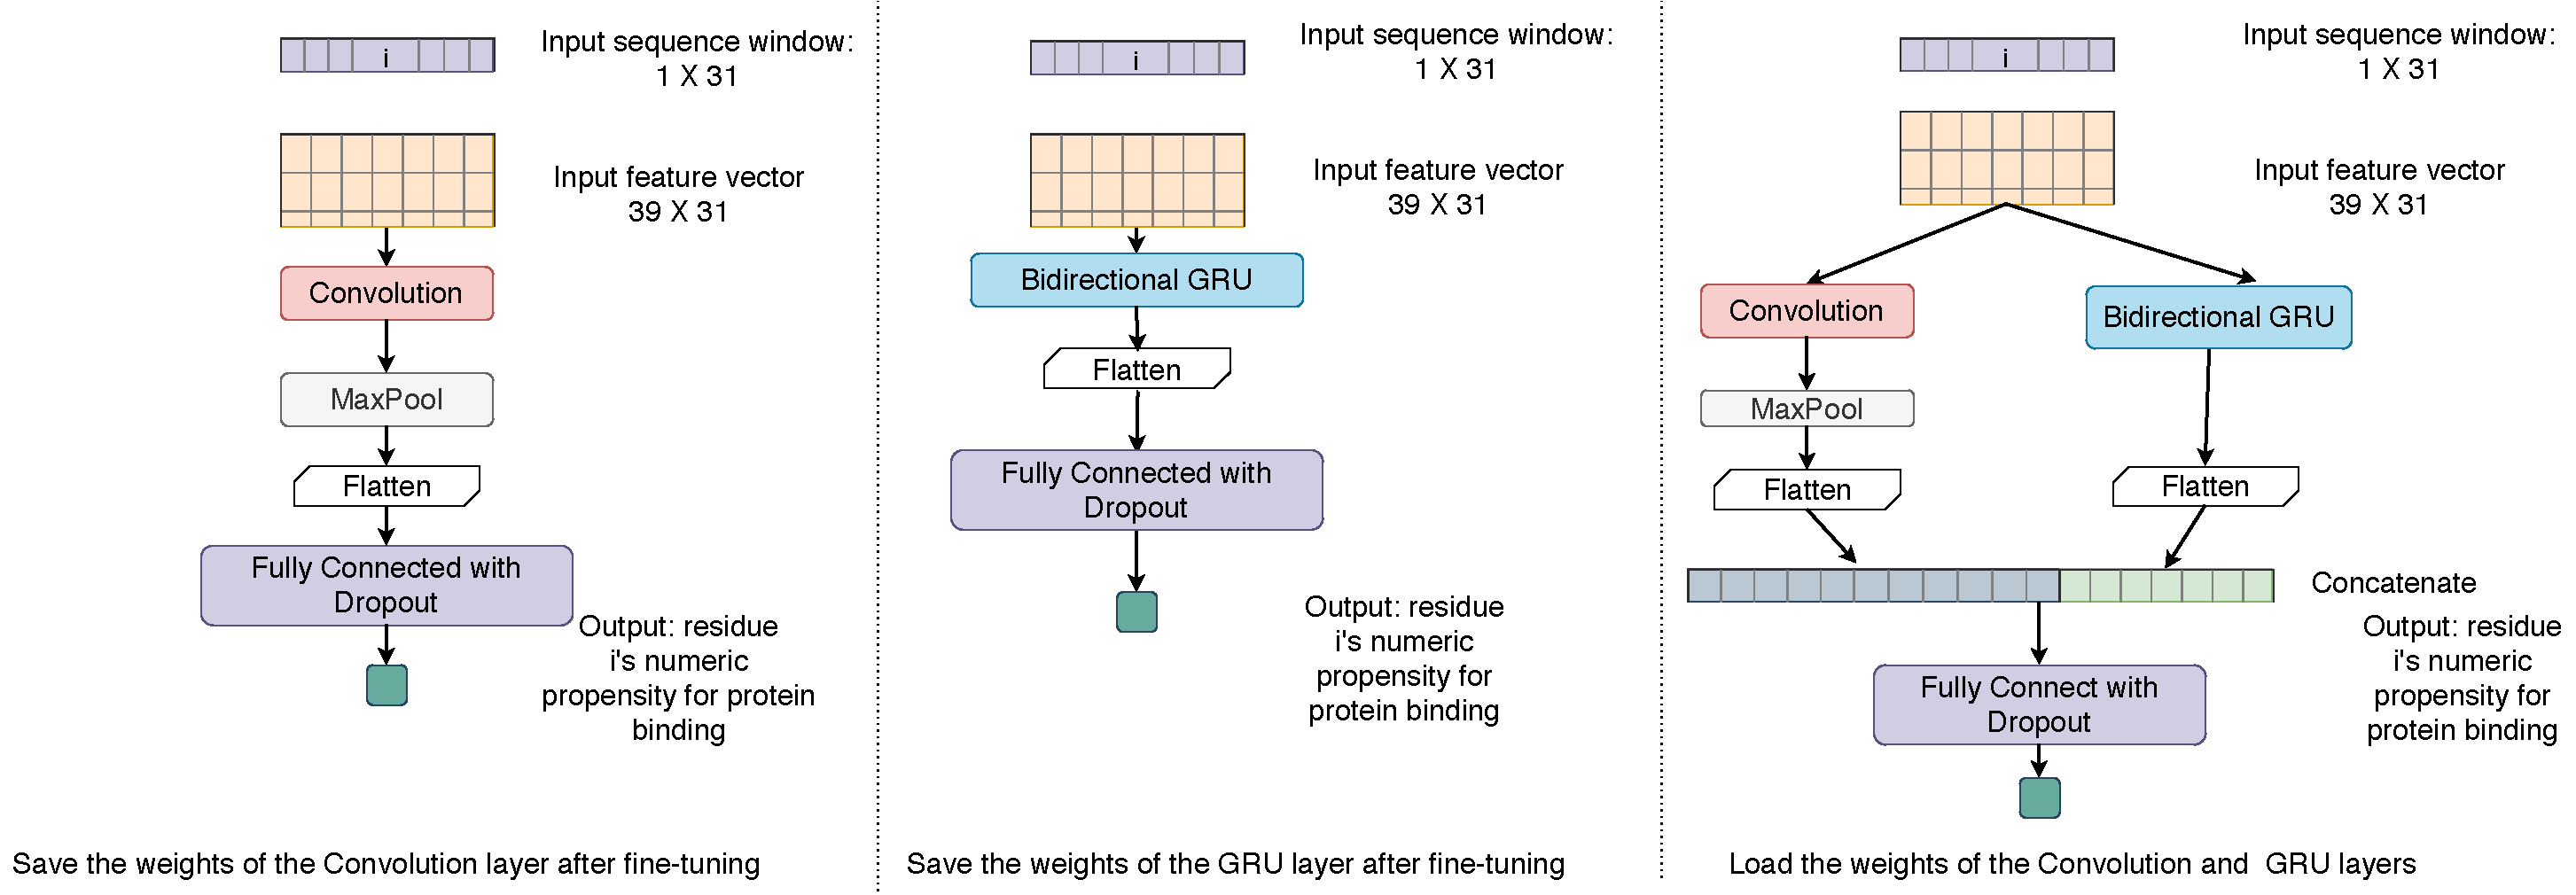
\includegraphics[width=\textwidth]{Model_architecture.pdf}
  \caption{\textbf{The architecture of DELPHI.} Left: the CNN component of the model. Middle: the RNN component of the model. Right: The ensemble model. 
  \label{fig_architecture}}
\end{figure*}

Another very useful characteristic of the model is its many-to-one structure, meaning that the information of many residues are used to prediction the binding propensity of the centered single residue. As illustrated in Fig. \ref{fig_many2one}, for each amino acid as the prediction target, a window of size 31, centred on the amino acid position, is used to collect information from the neighbouring 30 residues to help the prediction. A sliding window is used to capture each 31-mer. The size 31 is determined experimentally. The beginning and the ending part of the sequence are padded with zeros. The many-to-one structure has two advantages. Firstly, it serves as a data augmentation technique. Deep learning models need large amount of data to train, and comparing to image classifiers, models in proteomics have access to orders of magnitude less data. Using each residue multiple times during the training process helps the model learn better. Secondly, it makes the model more robust. The lengths of protein sequence vary from less than one hundred to several thousand, and most a many-to-many models have a fixed input length of near 500. During training, sequences around length 500 are often picked. However, during testing, input sequences are random and need to be either padded or cut into pieces. The different average lengths between training and testing could potentially make the model less general. 
\begin{figure*}
\centering
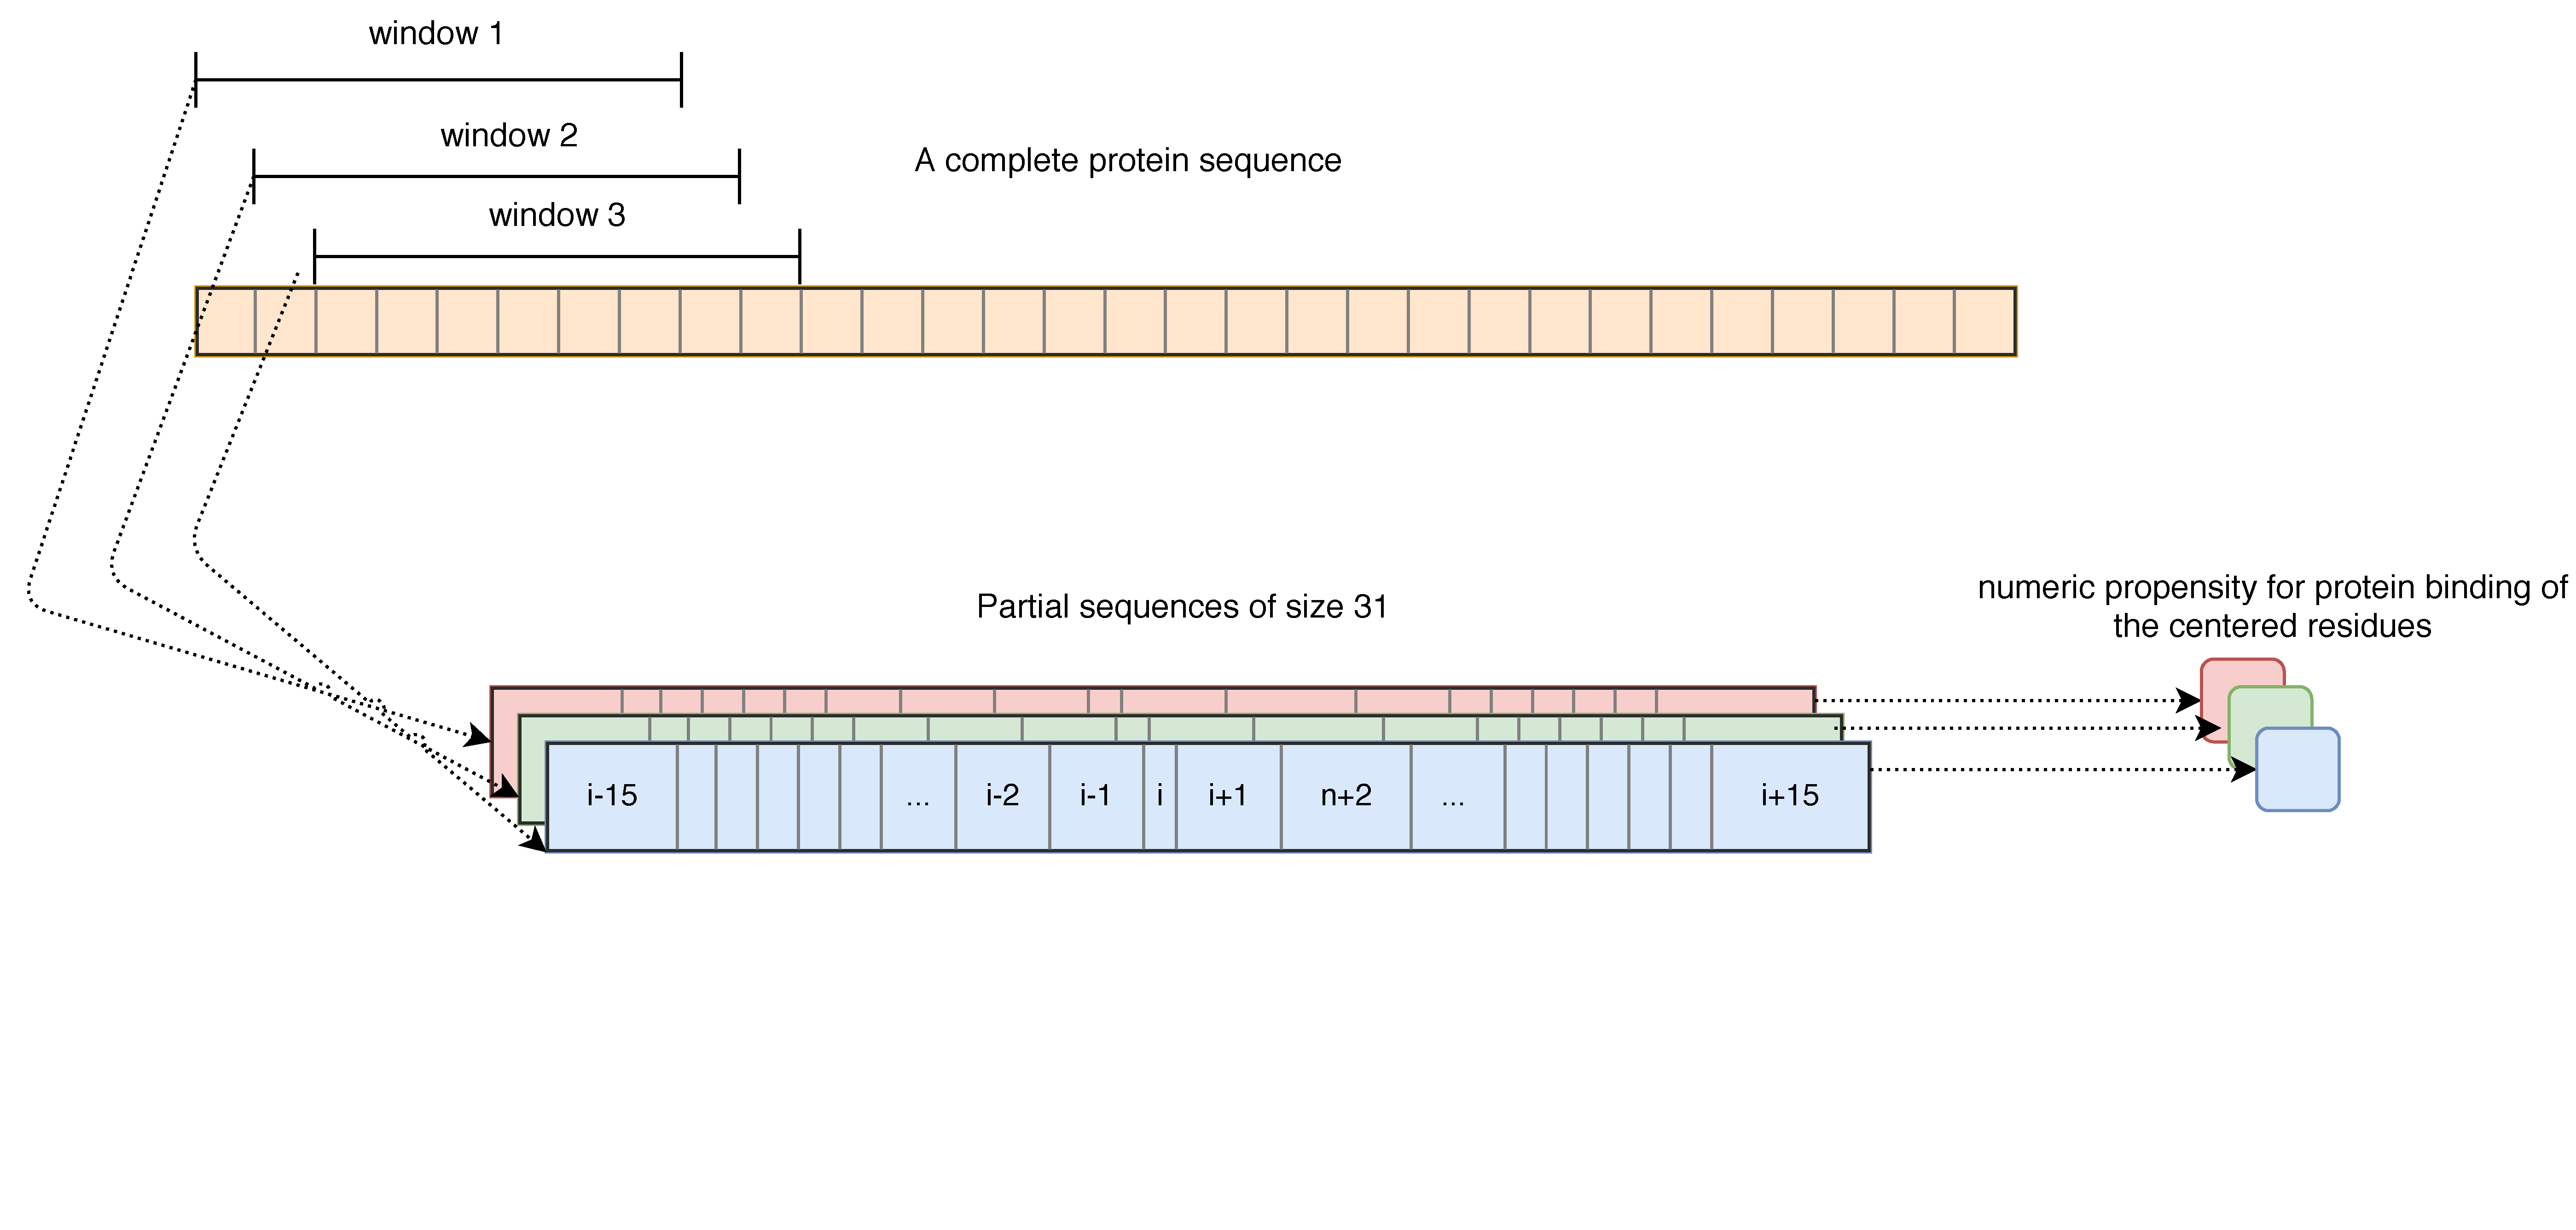
\includegraphics[width=\textwidth]{many_2_one.pdf}
  \caption{\textbf{The many-to-one prediction.} Sliding windows of size 31, stride 1 are put on top of an input protein sequence. Each time, a sub-sequence of length 31 is extracted. The model predicts the protein-binding propensity of the middle amino acid for each sub-sequence.
  \label{fig_many2one}}
\end{figure*}

\subsubsection{Architecture of the CNN network}
The CNN model one has a concise structure: one convolution layer, one maxpooling layer, one flatten layer, and two fully connected layers. For each input sub-sequence of size 31, a 2D feature profile of size 39 by 31 is constructed. The 2D vector is reshaped into 3D and then passed to a convolution 2D layer, followed by a maxpooling layer. The intuition of using the convolution and maxpooling layers is that a 2D protein profile vector can be considered as an image with one channel, and the CNN model captures the combination of several features in a partial image. The results are flattened and then fed into two fully connected layers with dropout for regularization. The last fully connected layer has one unit with activation function sigmoid, so that the output is a single value between 0 to 1. The higher the value, the more confident the CNN model claims that the residue is a PPI binding site.

\subsubsection{Architecture of the RNN network}
The RNN component has the following structure: one bidirectional GRU layer, one flatten layer, and two fully connected layers. Similar to the CNN component, a 2D feature profile of size 39 by 31 is built for each 31-mer. The feature profile is passed to a bidirectional gated recurrent units (GRU) layer with the intention to memories the dependency and relationship among the 31 residues. We set the GRU layer to return a whole sequence as opposed to return a single value. The results are flattened and fed into two fully connected layers with dropout. The output of the RNN network is also a single value between 0 to 1.

\subsubsection{Architecture of the ensemble network} \label{section_ensemble}
The final model combines the core layers of the above mentioned CNN and RNN models and tries to further extract essential information of protein binding. The ensemble network takes a sequence of length 31 as its input. Similar to the CNN and RNN components, a 39 by 31 feature vector is constructed and passed to both a convolution layer and a bidirectional GRU layer. The output of the convolution layer is passed on to a maxpool layer and then flattened. The GRU output is also flattened. Then the outputs of the two flatten layers are concatenated and passed on to two fully connected layers with dropout. The last fully connected layer has one output unit with a sigmoid activation function, so the final output is a single value between 0 to 1, indicating the propensity of being binding sites. This is the final output of the entire model. 

Fine tuning is used in this ensemble model. The convolution layer in the CNN network and the bidirectional GRU layer in the RNN network are tuned separated using the same training/validation dataset. After achieving the best performance on the CNN and the RNN components, the weights of the convolution and the GRU layer are saved to files. In the ensemble model, the convolution and the GRU layer load the saved weights from the file and freeze the weights, so that during the process of training, the convolution and the GRU layer stay unchanged. Training and validation data are used again only to train the fully connected layers in the ensemble model.

\subsection{Implementation}
The program is written in Keras \citep{chollet2015keras} (Python 3.5.2) with TensorFlow GPU \citep{tensorflow2015-whitepaper} back end. All features are computed from sequence only. We alleviate the burden of feature computation from users by providing all computation programs and a pipeline script. We ease the system configuration process by providing users a pip package list which enables one-command installation. 

Classifying protein binding residue is an imbalanced problem. To cope with that, different class weights \citep{ting2002instance} are assigned to the positive and negative samples, so that the model pays more attention to the minority class, which is the binding sites.  The values are determined by the inverse of the class distribution in the training datasets. In our program, the weights are 0.55 and 4.97 for the non-binding and binding sites respectively. 

During training, we shuffle the data before each epoch. Since the sliding window is used to extract each 31-mer, adjacent data entries are very similar; only the first and the last residue differ from the previous and the next data entry. Shuffling the whole training data diversifies the input in each batch. We experimentally trained the model with and without data shuffling, and shuffling the data rendered better predictions. 

\subsection{Parameter tuning}
\textcolor{\myColor}{Parameters and hyper-parameters are chosen empirically based on the training dataset while applying early stopping \citep{prechelt1998early} on the validation set.} Early stopping halts the training process when a performance drop on the validation set is detected. This is to avoid overfitting the training dataset. We chose all parameters with the purpose to maximize area under the precision-recall curve (AUPRC) of the training data. All testing results are then carried using the already tuned model. All parameters and hyper-parameters used in this model are shown in Table \ref{tab_parameter}. 
The DELPHI model takes 2.1 hours to train the CNN component, 0.5 hour to train the RNN component and 1.3 hours to train the ensemble model on a Linux (Ubuntu 16.04) machine with 24 CPUs (Intel Xeon v4, 3.00GHz), 256GB memory, and a Nvidia Tesla K40c GPU.

% Table generated by Excel2LaTeX from sheet 'Sheet1'
\begin{table}[H]
  \centering
  \caption{Parameters used in DELPHI. Parameters are divided into four groups: CNN, RNN, ensemble model, and hyper-parameters.}
    \begin{tabular}{@{}p{4.4cm}r@{}}
    \toprule
    Parameter & Value \\
    \midrule
    Epoch in CNN & 8 \\
    Kernel size in CNN & 5 \\
    Stride in CNN & 1 \\
    Padding in CNN & valid \\
    Number of filters in CNN & 64 \\
    Fully connected unit in CNN & 64, 1 \\
    \hline
    Epoch in RNN & 9 \\
    GRU unit & 32 \\
    Fully connected unit in RNN & 64, 1 \\
    \hline
    Epoch in ensemble & 5 \\
    Fully connected unit in ensemble & 96, 1 \\
    \hline
    Batch size & 1024 \\
    Dropout rate & 0.3 \\
    Optimizer & Adam ($\beta_1=0.9, \beta_2=0.999$) \\
    Patience in early stop & 4 \\
    Loss function & binary cross entropy \\
    Learning rate & 0.002 \\
    \bottomrule
    \end{tabular}%
  \label{tab_parameter}%
\end{table}%

% \enlargethispage{6pt}
\end{methods}

\section{Results}
\subsection{Competing methods}
We have comprehensively compared DELPHI with nine state-of-the-art machine learning based methods. The methods are selected using the following criteria. First, the program is a sequence-based method as sequence information is readily available for most proteins. Second, the program is available in the form of source code or web server. Lastly, the program takes in any input sequence in FASTA format and produces the results on an average-length protein within thirty minutes. Following these criteria, DLpred \citep{zhang2019sequence}, SCRIBER \citep{zhang2019scriber}, SSWRF \citep{wei2016protein}, SPRINT \citep{taherzadeh2016sequence}, CRF-PPI \citep{wei2015cascade}, LORIS \citep{dhole2014sequence}, SPRINGS \citep{singh2014springs}, PSIVER \citep{murakami2010applying}, and SPPIDER \citep{porollo2007prediction} are selected.

\textcolor{\myColor}{Ideally, we would like to have every program trained on sequences of less than 25\% similarity with any testing datasets, but all competing programs are either pre-trained or work as a web server, so there may be some level of similarities for them. Although we had to use other programs as is, we selected DELPHI's training dataset to ensure it meets similarity criteria. Notice that this is to the disadvantage of DELPHI.}

 The most recent two programs, DLPred and SCRIBER, use 5719 and 843 training proteins respectively. The training dataset of DLPred is obtained from CullPDB datasets \citep{wang2003pisces} and further filtered by the authors. The SCRIBER training dataset is originally from the BioLip database. This dataset contains also protein binding information with DNA, RNA, and ligand, which is used by SCRIBER.

\subsection{Evaluation scheme}
Similar to previous studies, we use sensitivity, specificity, precision, accuracy, F1-score (F1), Matthews correlation coefficient (MCC), area under the receiver operating characteristic curve (AUROC), and area under the precision-recall curve (AUPRC) to measure the prediction performance. All programs output a prediction value for each amino acid, and thus the receiver operating characteristic (ROC) curve and the precision-recall (PR) curve can be drawn. AUROC and AUPRC are computed using Scikit-learn~ \citep{scikit-learn}. Area under curves are threshold independent and convey an overall performance measurement of a program. The rest of the metrics are calculated using a binding threshold which is determined after obtaining the prediction scores from each program. Since each program's output is of different scale, for each program, we pick the threshold such that for a given testing dataset, the number of predicted scores above the threshold is equal to the real number of binding sites in the dataset. Binding site prediction is a highly imbalanced task, the area under the PR curve and MCC are better indications of the performance as it emphasises more on the minority class while ROC curve pays attention to both minority and the majority class \citep{andluis2016survey} \citep{saito2015precision}.  

The formulas for calculating the metrics are as follows, where true positives ($TP$) and true negatives ($TN$) are the correctly predicted binding sites and non-binding sites, respectively, and false positives ($FP$) and false negative ($FN$) are incorrectly predicted binding sites and non-binding sites, respectively:
\[
\begin{array}{ll}
\displaystyle{\textit{Sensitivity} = \frac{TP}{TP+FN},} & \displaystyle{\textit{Specificity} = \frac{TN}{TN+FP},} \smallskip \\ 
\displaystyle{\textit{Precision} = \frac{TP}{TP + FP},} & \displaystyle{\textit{Accuracy}=\frac{TP+TN}{TP+FN+TN+FP},}\smallskip \\ 
\multicolumn{2}{l}{\displaystyle{F1=2\times \frac{\textit{Sensitivity}\times \textit{Precision}}{\textit{Sensitivity}+\textit{Precision}}},}\smallskip\\
\multicolumn{2}{l}{\displaystyle{MCC\!=\!\frac{TP \times TN - FN \times FP}{\sqrt{(TP\!+\!FP)\!\times\! (TP\!+\!FN)\! \times \!(TN\!+\!FP)\!\times\!(TN\!+\!FN)}}}.}\\
\end{array}
\]

\subsection{Comparative assessment of predictive performance}
\subsubsection{Performance comparison on Dset\_448 and Dset\_355}
We first compare the DELPHI model with eight programs on Dset\_448. This dataset is the largest and the most recently published. As shown in Table \ref{tab_comp_448_355}, DELPHI surpasses competitors in all metrics with an improvement of 17.4\%, 18.3\%, and 3.08\% on AUPRC, MCC, and AUROC respectively comparing to the second best program SCRIBER.

\textcolor{\myColor}{As mentioned earlier, Dset\_448 cannot be used for DLPred, so we include a comparison of all programs on Dset\_355. As shown in Table \ref{tab_comp_448_355}, the performance of DLPred is very similar to the second best predictor, SCRIBER.  DELPHI still surpasses the second best program by 18.5\% and 20.9\% on AUPRC and MCC.  }

\subsubsection{Performance comparison on Dset\_186, Dset\_164, and Dset\_72}\label{section_four_tests}
\textcolor{\myColor}{To further compare DELPHI with other programs, we used another three previously published datasets: Dset\_186, Dset\_164, and Dset\_72. Based on the availability and usability, We ran SPPIDER, PSIVER, CRFPPI, SCRIBER, DELPred, and DELPHI on them. Note that SSWRF, CRFPPI, and PSIVER use Dset\_186 as their training datasets, so these three programs are excluded on Dset\_186. As shown in Table \ref{tab_ds186_164_72}, in general, the performance rank is the very similar to the ones in Dset\_448 and Dset\_355.}

% \clearpage
\begin{table}[H]
  \centering
  \caption{\textcolor{\mySecondColor}{Performance comparison on Dset\_448 and Dset\_355. Programs are sorted in ascending order by AUPRC. Bold fonts indicate the best results. The evaluation of the programs marked with ${}^*$ is by  \cite{zhang2019scriber}.}}
    % Table generated by Excel2LaTeX from sheet 'Sheet2'
    \begin{tabular}{@{}l@{\ }*{8}{r}}
    \toprule
    \multicolumn{1}{@{}l}{Predictor} & \multicolumn{1}{c}{$\!$Sens.} & \multicolumn{1}{c}{Spec.} & \multicolumn{1}{c}{Prec.} & \multicolumn{1}{c}{Acc.} & \multicolumn{1}{c}{F1} & \multicolumn{1}{c}{MCC} & \multicolumn{1}{c}{$\!\!\!$AUROC$\!\!\!$} & \multicolumn{1}{c@{}}{$\!$AUPRC} \\
    \hline
    \multicolumn{9}{c}{Dset\_448} \\
    \hline
       SPPIDER* & 0.202 & 0.870 & 0.194 & 0.781 & 0.198 & 0.071 & 0.517 & 0.159 \\
    SPRINT* & 0.183 & 0.873 & 0.183 & 0.781 & 0.183 & 0.057 & 0.570 & 0.167 \\
    PSIVER* & 0.191 & 0.874 & 0.191 & 0.783 & 0.191 & 0.066 & 0.581 & 0.170 \\
    SPRINGS* & 0.229 & 0.882 & 0.228 & 0.796 & 0.229 & 0.111 & 0.625 & 0.201 \\
    LORIS* & 0.264 & 0.887 & 0.263 & 0.805 & 0.263 & 0.151 & 0.656 & 0.228 \\
    CRFPPI* & 0.268 & 0.887 & 0.264 & 0.805 & 0.266 & 0.154 & 0.681 & 0.238 \\
    SSWRF* & 0.288 & 0.891 & 0.286 & 0.811 & 0.287 & 0.178 & 0.687 & 0.256 \\
    SCRIBER & 0.334 & 0.896 & 0.332 & 0.821 & 0.333 & 0.230 & 0.715 & 0.287 \\
    DELPHI & \textbf{0.371} & \textbf{0.901} & \textbf{0.371} & \textbf{0.829} & \textbf{0.371} & \textbf{0.272} & \textbf{0.737} & \textbf{0.337} \\
    \hline
    \multicolumn{9}{c}{Dset\_355} \\
    \hline
    SPPIDER & 0.180 & 0.889 & 0.180 & 0.804 & 0.180 & 0.068 & 0.515 & 0.138 \\
    SPRINT & 0.168 & 0.886 & 0.167 & 0.801 & 0.168 & 0.054 & 0.571 & 0.150 \\
    PSIVER & 0.178 & 0.888 & 0.177 & 0.803 & 0.177 & 0.065 & 0.583 & 0.155 \\
    SPRINGS & 0.211 & 0.892 & 0.210 & 0.811 & 0.211 & 0.103 & 0.608 & 0.178 \\
    LORIS & 0.242 & 0.896 & 0.240 & 0.818 & 0.241 & 0.137 & 0.637 & 0.203 \\
    CRFPPI & 0.247 & 0.897 & 0.245 & 0.819 & 0.246 & 0.143 & 0.662 & 0.214 \\
    SSWRF & 0.268 & 0.901 & 0.268 & 0.825 & 0.268 & 0.168 & 0.667 & 0.228 \\
    SCRIBER & 0.322 & 0.908 & 0.322 & 0.838 & 0.322 & 0.230 & 0.719 & 0.275 \\
    DLPred & 0.308 & 0.906 & 0.308 & 0.835 & 0.308 & 0.214 & 0.724 & 0.272 \\
    DELPHI & \textbf{0.364} & \textbf{0.914} & \textbf{0.364} & \textbf{0.848} & \textbf{0.364} & \textbf{0.278} & \textbf{0.746} & \textbf{0.326} \\
    \hline
    \end{tabular}%
  \label{tab_comp_448_355}%
\end{table}%
\begin{table}[H]
  \centering
  \caption{\textcolor{\mySecondColor}{Performance comparison on Dset\_186, Dset\_164, and Dset\_72 using the same metrics. Bold fonts indicate the best results.}}
    \begin{tabular}{@{}l@{\ }*{8}{r}}
    \toprule
    \multicolumn{1}{@{}l}{Predictor} & \multicolumn{1}{c}{$\!$Sens.} & \multicolumn{1}{c}{Spec.} & \multicolumn{1}{c}{Prec.} & \multicolumn{1}{c}{Acc.} & \multicolumn{1}{c}{F1} & \multicolumn{1}{c}{MCC} & \multicolumn{1}{c}{$\!\!\!$AUROC$\!\!\!$} & \multicolumn{1}{c@{}}{$\!$AUPRC} \\
    \hline
    \multicolumn{9}{c}{Dset\_186} \\
    \hline
    SPPIDER & 0.194 & 0.848 & 0.186 & 0.748 & 0.190 & 0.041 & 0.499 & 0.165 \\
    SCRIBER & 0.279 & 0.870 & 0.279 & 0.780 & 0.279 & 0.150 & 0.647 & 0.246 \\
    DLPred & 0.320 & 0.878 & 0.320 & 0.793 & 0.320 & 0.198 & 0.694 & 0.290 \\
    DELPHI & \textbf{0.351} & \textbf{0.884} & \textbf{0.351} & \textbf{0.803} & \textbf{0.351} & \textbf{0.235} & \textbf{0.710} & \textbf{0.319} \\

    \hline
    \multicolumn{9}{c}{Dset\_164} \\
    \hline
    SPPIDER & 0.264 & 0.828 & 0.253 & 0.726 & 0.258 & 0.090 & 0.528 & 0.220 \\
    PSIVER & 0.217 & 0.826 & 0.216 & 0.716 & 0.216 & 0.043 & 0.554 & 0.205 \\
    CRFPPI & 0.280 & 0.841 & 0.280 & 0.739 & 0.280 & 0.121 & 0.608 & 0.267 \\
    SSWRF & 0.266 & 0.838 & 0.266 & 0.734 & 0.266 & 0.103 & 0.606 & 0.243 \\
    SCRIBER & 0.327 & 0.851 & 0.327 & 0.756 & 0.327 & 0.179 & 0.657 & 0.301 \\
    DLPred & 0.338 & 0.854 & 0.338 & 0.760 & 0.338 & 0.192 & 0.672 & 0.330 \\
    DELPHI & \textbf{0.352} & \textbf{0.857} & \textbf{0.352} & \textbf{0.765} & \textbf{0.352} & \textbf{0.209} & \textbf{0.685} & \textbf{0.332} \\
    \hline
    \multicolumn{9}{c}{Dset\_72} \\
    \hline
    SPPIDER & 0.188 & 0.898 & 0.179 & 0.823 & 0.183 & 0.084 & 0.522 & 0.134 \\
    PSIVER & 0.152 & 0.899 & 0.152 & 0.820 & 0.152 & 0.052 & 0.604 & 0.141 \\
    CRFPPI & 0.248 & 0.911 & 0.248 & 0.840 & 0.248 & 0.158 & 0.669 & 0.200 \\
    SSWRF & 0.246 & 0.911 & 0.246 & 0.840 & 0.246 & 0.157 & 0.678 & 0.198 \\
    SCRIBER & 0.232 & 0.909 & 0.232 & 0.837 & 0.232 & 0.141 & 0.680 & 0.198 \\
    DLPred & 0.246 & 0.901 & 0.246 & 0.826 & 0.246 & 0.148 & 0.688 & 0.215 \\
    DELPHI & \textbf{0.274} & \textbf{0.914} & \textbf{0.274} & \textbf{0.847} & \textbf{0.274} & \textbf{0.189} & \textbf{0.711} & \textbf{0.237} \\
    \hline
\label{tab_ds186_164_72}
    \end{tabular}%
\end{table}%




\textcolor{\myColor}{
DELPHI clearly outperforms the competitors in all metrics on all datasets although it shares the least similarities to the testing datasets.  The AUPRC is improved by 10.0\%, 0.6\%, 10.2\% comparing to the second best program on each dataset. The improvement on MCC are 18.7\%, 8.9\%, 27.7\% on each dataset. 
}

\subsection{Ablation study}

\subsubsection{Feature evaluation}
We conducted an experiment to show that all twelve feature are useful. We pruned one feature each time, and the remaining eleven features are used to train and then evaluate the DELPHI model. As shown in Fig. \ref{fig_remove_each_feature}, the performance decreases with the removal of any feature, showing that there are no redundant features. It is perhaps expected that  removing PSSM creates the biggest performance drop, but our newly introduced features, HSP, ProtVec1D, and Position are shown to be  very useful as well. 

\textcolor{\myColor}{
\subsubsection{The evaluation of the model architecture and the novel features}
To show that the ensemble architecture and the three novel features improve the performance, we evaluated the CNN, RNN, and the ensemble model separately on Dset\_448 with and without the three new features, a total of six tests. Training is done as before (section \ref{section_ensemble}). In Fig. \ref{fig_CNN_RNN_ensemble}, we plotted the value of AUPRC and MCC of the six tests. Clearly, the ensemble model outperforms the individual CNN and RNN models. Further, the improvement due to the three new features is even higher, with the weakest model, CNN, on 12 features outperforming the ensemble on 9 features. }

\subsubsection{Other explorations}
We also tried some other ideas that could be potentially interesting, such as representing the protein sequence with one-hot embedding or the original 100 dimensional ProtVec. Unfortunately the results did not surpass the existing sequence representation. Under-sampling non-binding residuals and over-sampling binding residuals resulted in unstable performance, related to the ratio of the testing datasets. For example the prediction on the highest binding residue ratio Dset\_164 was improved by the sampling methods but not on other datasets. Attention mechanism also failed to improve the results. In terms of the network architecture, LSTM, 1D convolution, and combining the CNN and RNN network without training them separately have been tested. In the end we picked the reported architecture empirically. 

\begin{figure}
\centering
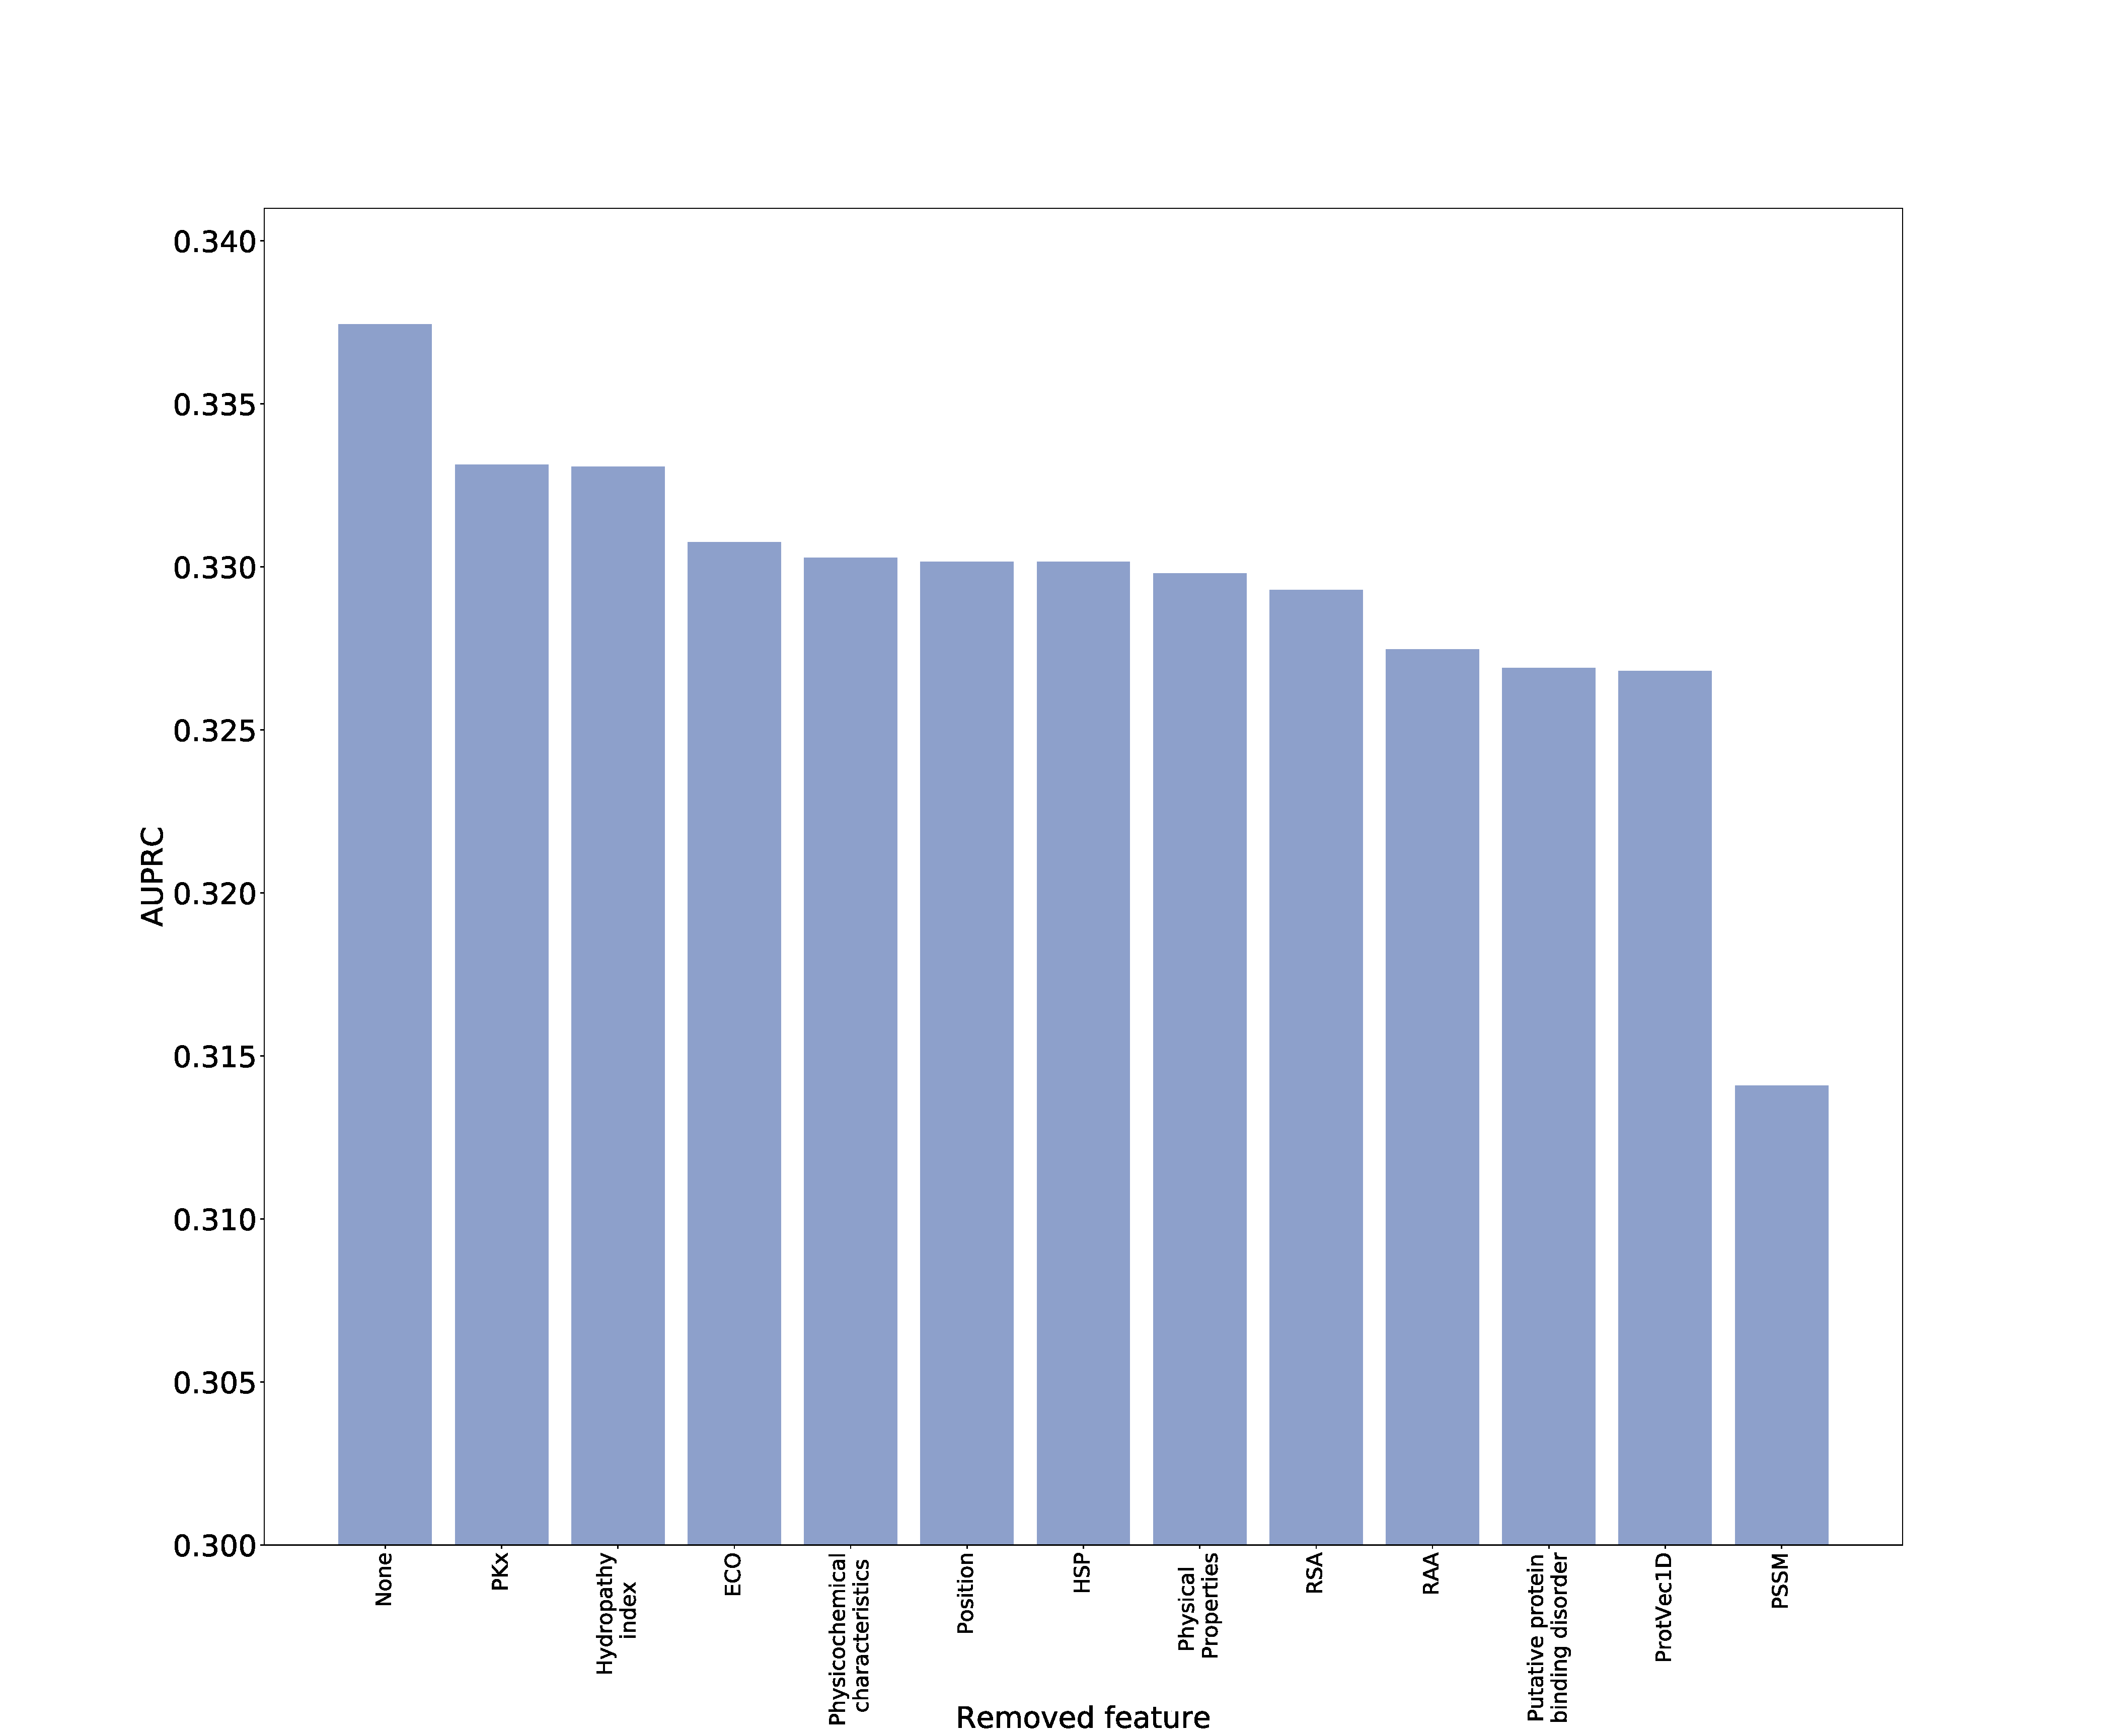
\includegraphics[width=\columnwidth]{remove_features_individually_Testing.pdf}
  \caption{\textbf{The areas under PR curves with the removal of one out of the twelve features on Dset\_448.} One feature is removed each time, and the DELPHI model is trained, validated, and tested using the remaining eleven features. The x-axis shows the removed features where 'None' indicates using all twelve features, and the y-axis is the AUPRC achieved. The features are sorted decreasingly by the AUPRC values. 
  \label{fig_remove_each_feature}}
\end{figure}

\begin{figure}
\centering
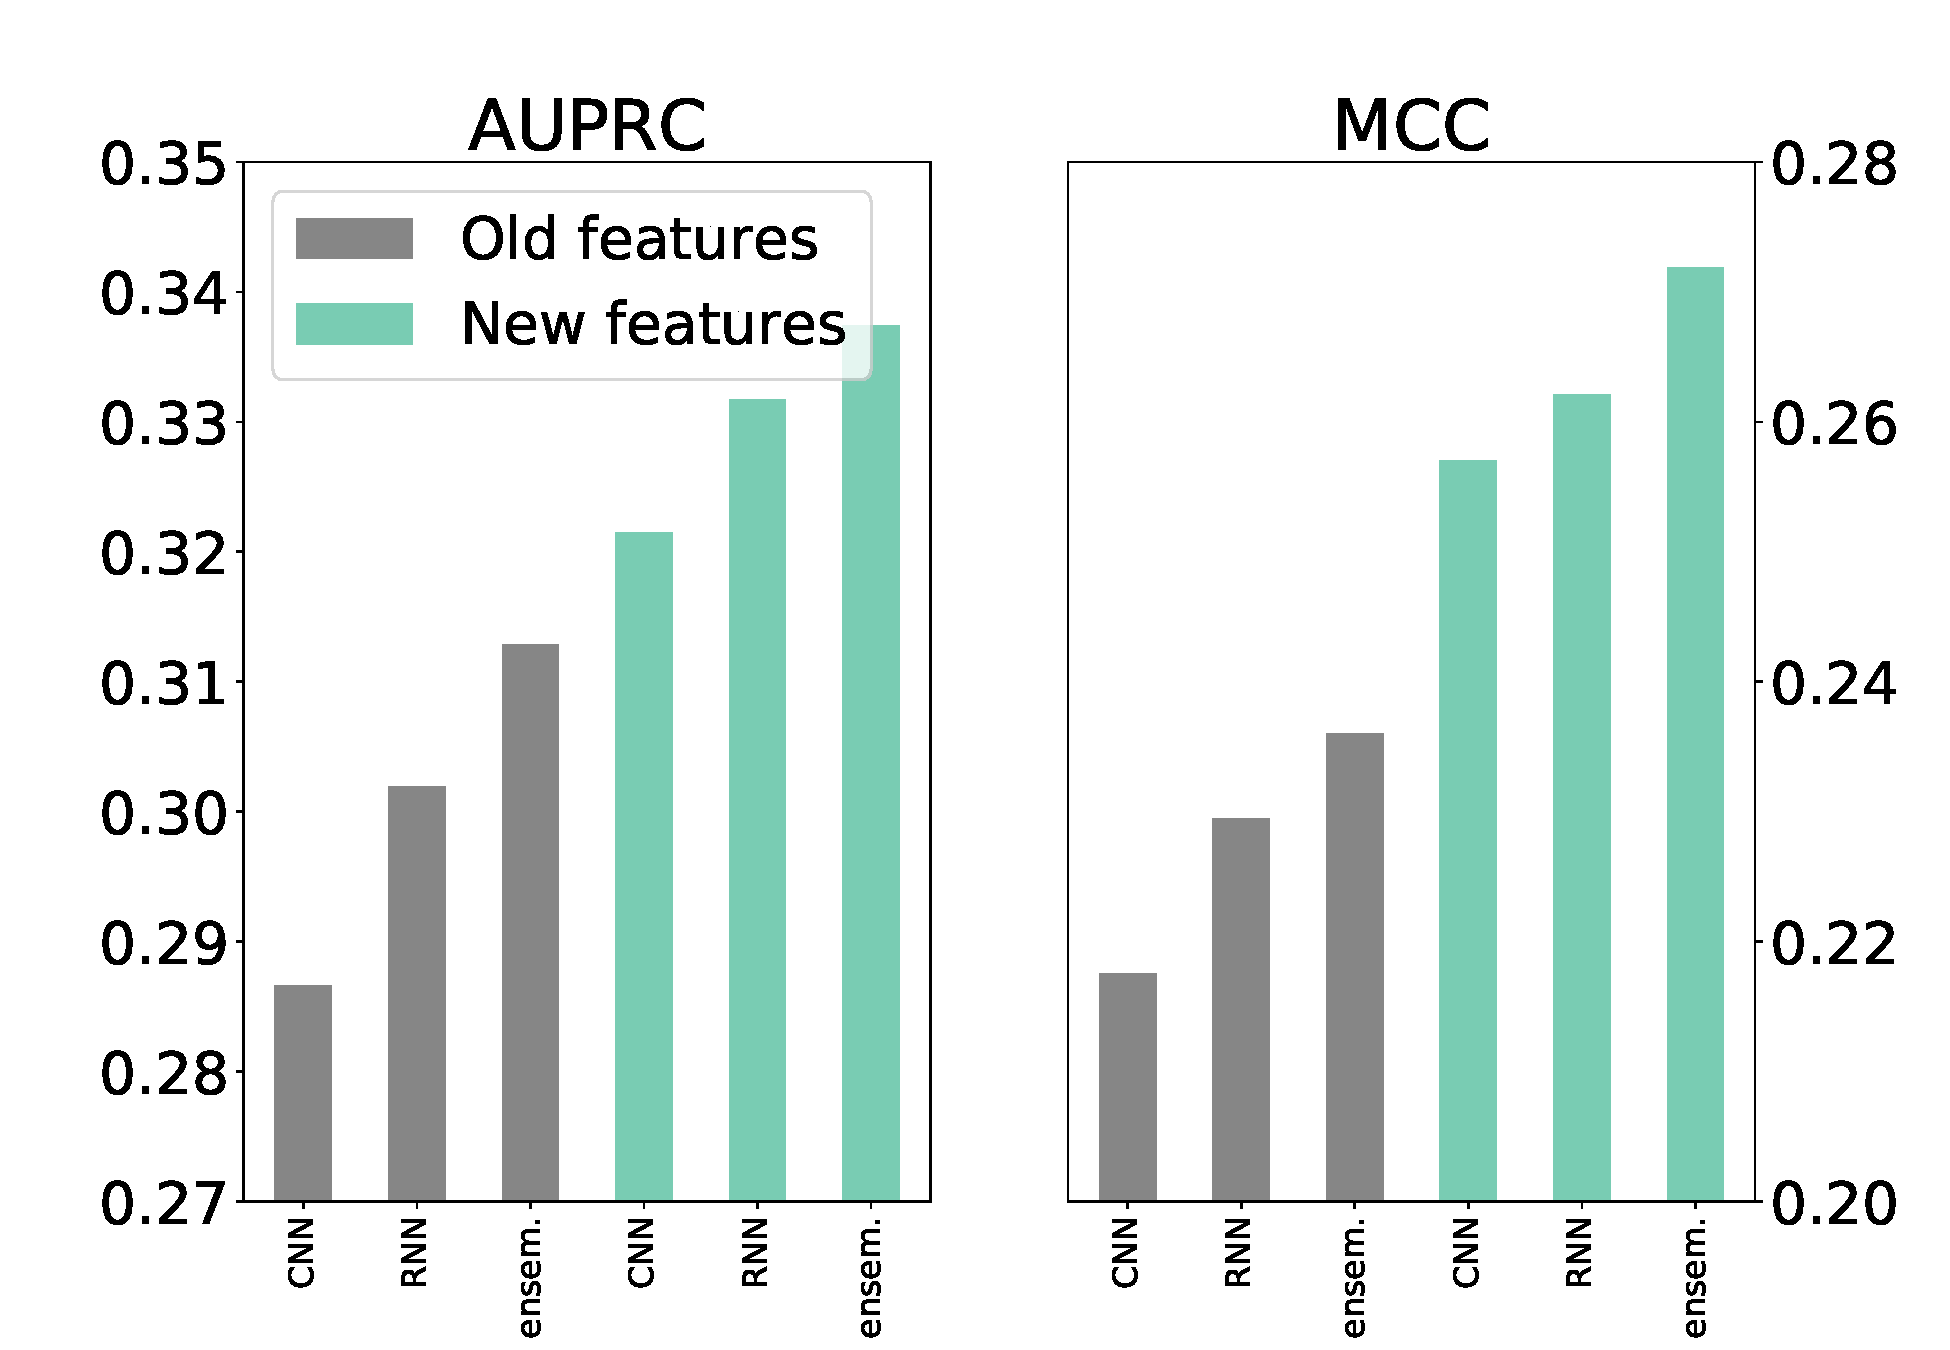
\includegraphics[width=\columnwidth]{CNN_RNN_ensemble.pdf}
  \caption{\textcolor{\myColor}{{The evaluation of the DELPHI model architecture and the three novel features.} The area under PR curves (left) and MCC (right) are plotted separately. Each plot contains the performance of using CNN, RNN, and the ensemble model on Dset\_448. Two different colors indicate with and without the three new features.}
  \label{fig_CNN_RNN_ensemble}}
\end{figure}


\begin{figure*}
\centering
\begin{tabular}{cc}
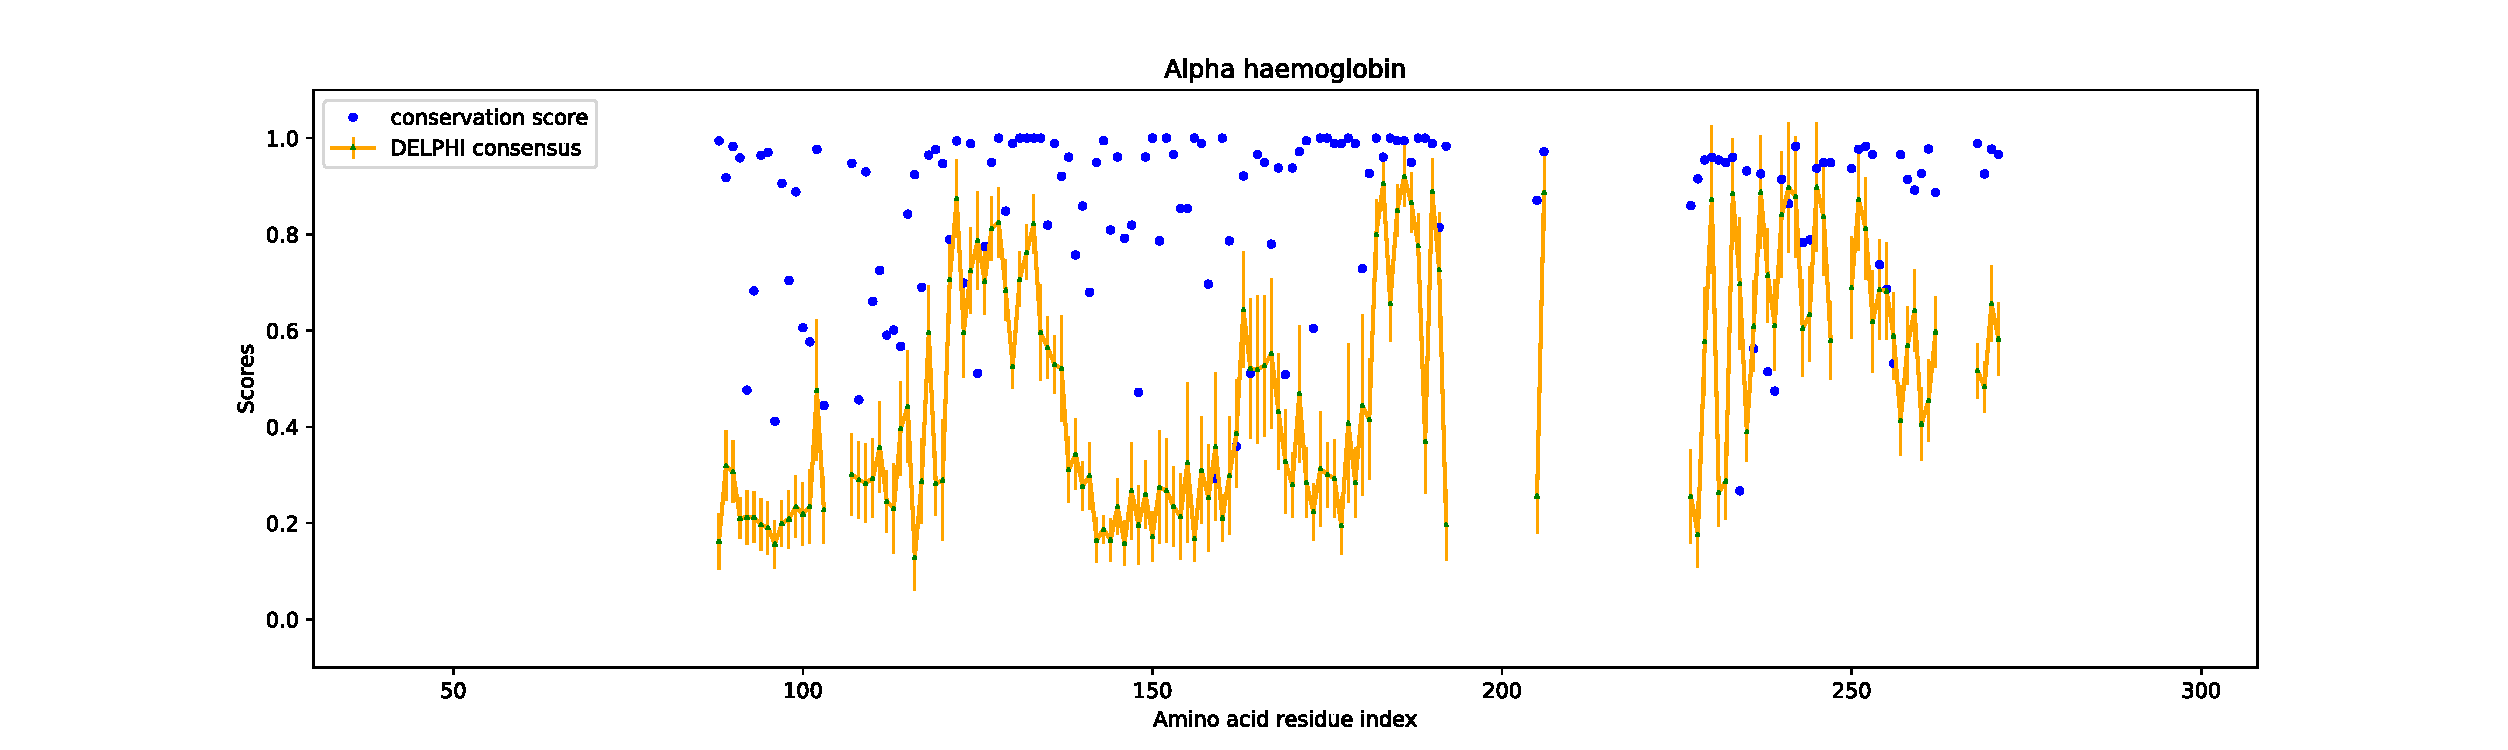
\includegraphics[height=2.55cm]{hemoglobin_top178_conservation.pdf} & 
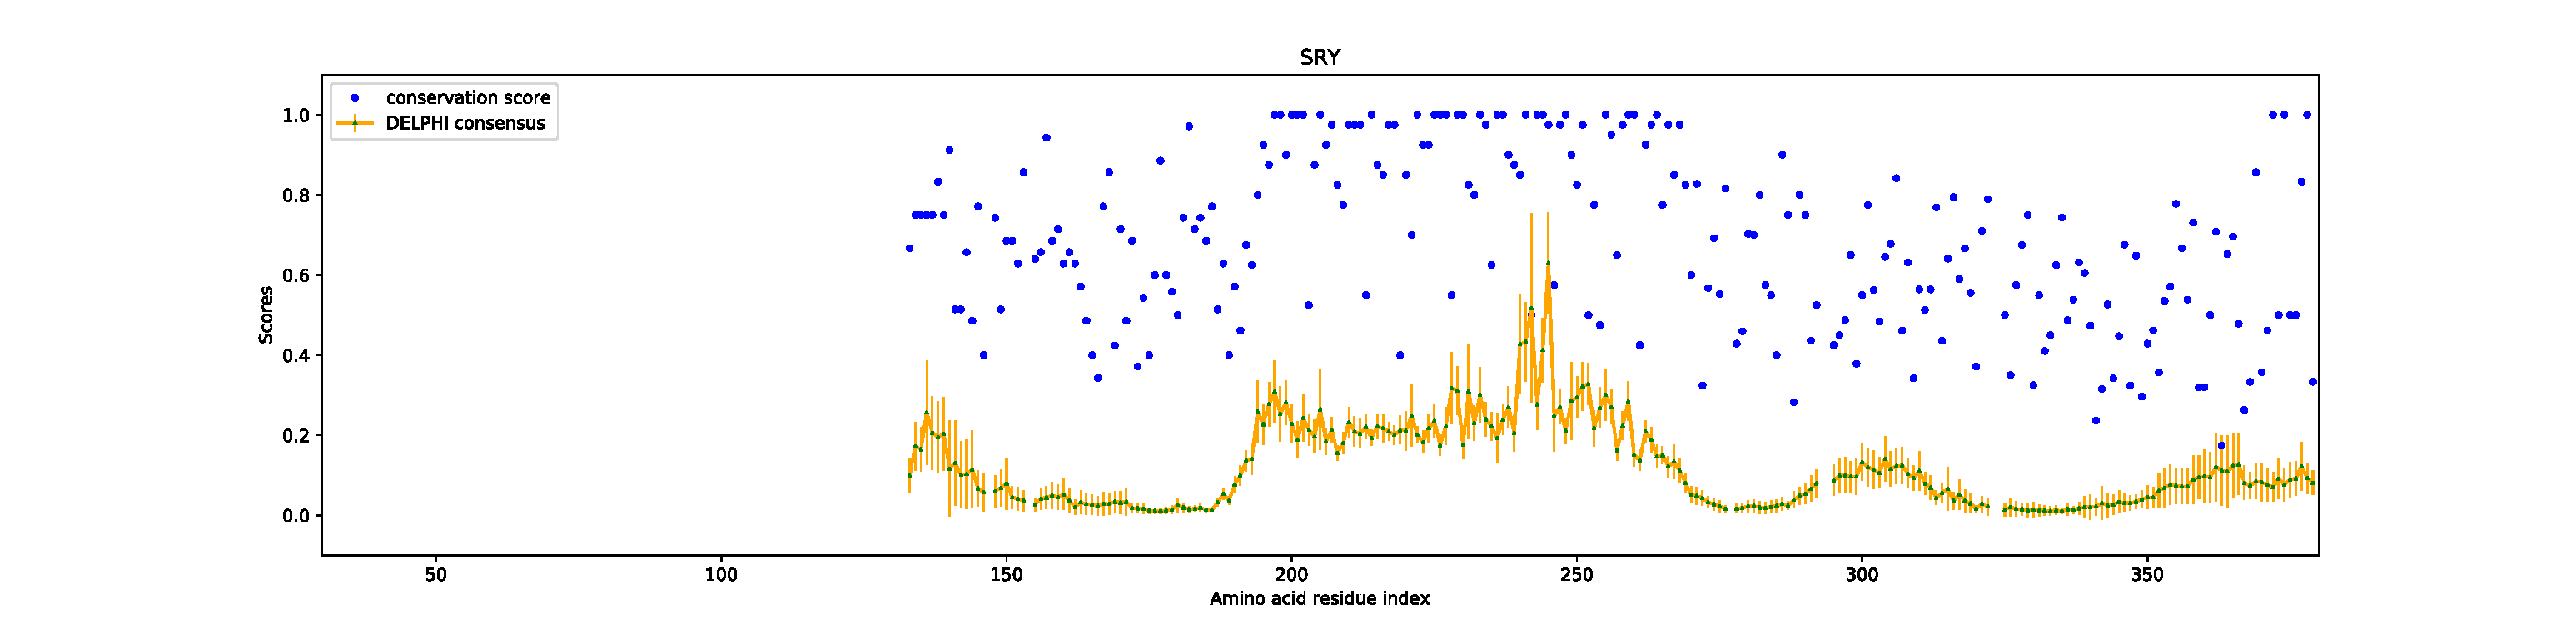
\includegraphics[height=2.55cm]{SRY_conservation.pdf}\\
\small (a) & \small (b)\\
\multicolumn{2}{c}{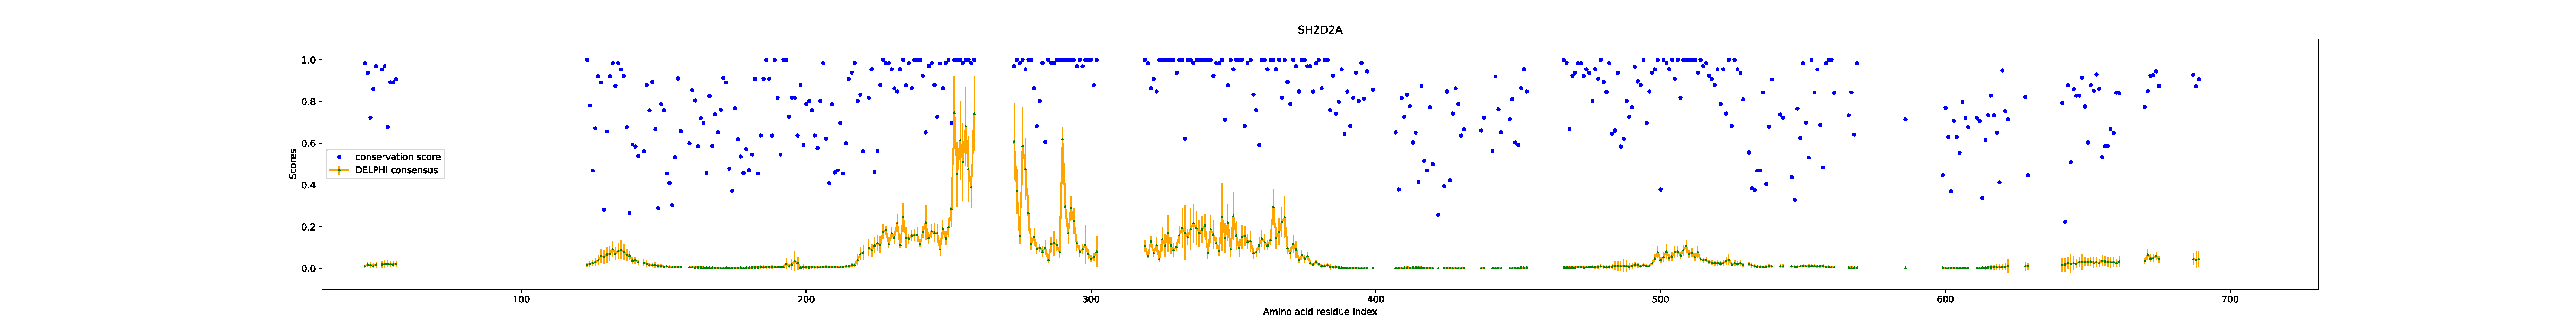
\includegraphics[height=2.55cm]{SH2_conservation.pdf}}\\
\multicolumn{2}{c}{\small (c)}
\end{tabular}
  \caption{\textcolor{\mySecondColor}{Three proteins were evaluated to compare the PPI
predicted by DELPHI (orange) with the degree of site-by-site conservation
(blue).  Only sites represented in ten or more taxa are included resulting
in some apparent gaps.  The proteins are (a) alpha haemoglobin, (b) SRY
and (c) SH2D2A.} 
  \label{fig_conservation_vs_sitePred}}
\end{figure*}


\subsection{\textcolor{\mySecondColor}{Application}}

\textcolor{\mySecondColor}{We analyzed three different proteins.  These are the transcription factor SH2D2A (399 amino acids in length), the alpha-subunit of the haemoglobin protein (142 amino acids in length) and the SRY protein (204 amino acids
in length).}

\textcolor{\mySecondColor}{For each protein, BLASTP was used to search for homologues.  The search was restricted to the refseq\_protein database to ensure good quality and
to proteins from mammalian organisms.  The SH2D2A sequences were further
limited to isoform X1 and the haemoglobins sequences were restricted to
proteins labelled as alpha subunits.  Sequences were aligned with MUSCLE
\citep{edgar2004muscle} and any sequences with unusually long protein distances
were further eliminated by hand.}

\textcolor{\mySecondColor}{This resulted in 66 homologous SH2D2A sequences, 178 homologous alpha
subunit haemoglobin sequences and 40 homolgous SRY sequences.  For each
site in the alignment of these proteins, the frequency of the most
conserved amino acid was recorded and compared to the PPI predicted by
DELPHI in Figure~\ref{fig_conservation_vs_sitePred}.  There are gaps in these figures since only aligned
sites present in more than 10 taxa were included in this comparison.}

\textcolor{\mySecondColor}{In general, Figure~\ref{fig_conservation_vs_sitePred}.a and Figure~\ref{fig_conservation_vs_sitePred}.c shows that the locations where
DELPHI predicted a high probability of a protein-protein interaction are
also the sites with a high degree of sequence conservation.  As expected
this correlation is not perfect since sequence conservation can occur
for many reasons other than PPI.  It will also be noted that the overall
degree of conservation in Figure~\ref{fig_conservation_vs_sitePred}.a for the alpha haemoglobin proteins is
much more conserved than for the other two proteins and is an indication
that these proteins are evolving slower.  Still PPI has a high probability
around 130aa, 185aa and 240aa but has a lower probability at the sites
around 175aa.  Similarly for sites around 350aa and 500aa in Figure~\ref{fig_conservation_vs_sitePred}.c
(protein SH2D2A) the PPI is low but the level of conservation is high.}

\textcolor{\mySecondColor}{The protein SRY in Figure~\ref{fig_conservation_vs_sitePred}.b binds to sites in the DNA rather
than to other proteins or internally.  This is the reason for the
high conservation around 190aa to 260aa.  Except for two sites the
probabilities predicted by DELPHI fluctuate around low values.}

\textcolor{\mySecondColor}{In general the data in Figure~\ref{fig_conservation_vs_sitePred} show that sites with a high probability
of PPI have a high degree of sequence conservation and indicate good
support for the validity of the method.  The opposite is not true.
Sequence conservation can occur for reasons other than the requirement
that the sites are constrained by protein-protein interactions.}



% According to the databases the interaction sites are ...
% 
%     Site            order(32,35..36,42..43,93,95..96,104,108,111..112,
%                     118..120,123..124,127,141..142)
%                     /site_type="other"
%                     /note="tetramer interface [polypeptide binding]"
%                     /db_xref="CDD:271278"
%     Site            order(33,43..44,59,62..63,66,84,88,98..99,102,137)
%                     /site_type="other"
%                     /note="heme binding site [chemical binding]"
%                     /db_xref="CDD:271278"
% 
% --------------------------------------------------------------
% 
% SRY is a sex-determining gene.  I was only able to find a smaller
% number of these genes where I thought the homology was clear.
% 
% In this case there are forty of them.  Sry is a little different in
% that it binds DNA.
% 
% SRY  Site            order(62,64..65,67..68,71..72,75,79,87,92,95,98,117)
%                      /site_type="DNA binding"
%                      /note="DNA binding site [nucleotide binding]"
%                      /db_xref="CDD:238684"
% 
% These sites should be conserved but might not show PPI.
% 
%


\subsection{Software availability}
\textcolor{\mySecondColor}{DELPHI is available both as a open sourced standalone software under the GPLv3 License and web server. The trained model, source code, and data processing pipeline are freely available at \texttt{github.com/lucian-ilie/DELPHI}. The web server is at  \texttt{www.csd.uwo.ca/\textasciitilde{}yli922/index.php}.
It facilitates use without programming skills. The user can input protein sequences and receive the prediction results via email. The PSSMs of all proteins in the testing datasets as well as the human proteome are pre-computed on the server. The average computation time for a protein of length 500 on the web server is 3 minuets if having pre-computed PSSM and 15 minutes wihtout pre-computed PSSM.
}


\section{Conclusion}
We have presented a new deep learning model and program DELPHI, for predicting PPI binding sites. We compared DELPHI with nine current state-of-the-art programs on five datasets and demonstrated that DELPHI has a higher prediction performance. There is still plenty room for improvement on this topic as the highest AUROC in all tests is 0.746. 
We hope that in the future, the model architecture, the usage of the three new features, and the many-to-one structure can be extended to predicting protein biding with other types of molecules, such as DNA, RNA, and ligand. Other deep learning techniques could be better used on this topic including better pre-trained embedding, better sampling methods for imbalanced problems in bioinformatics. 

% \begin{figure*}
% \centering
% 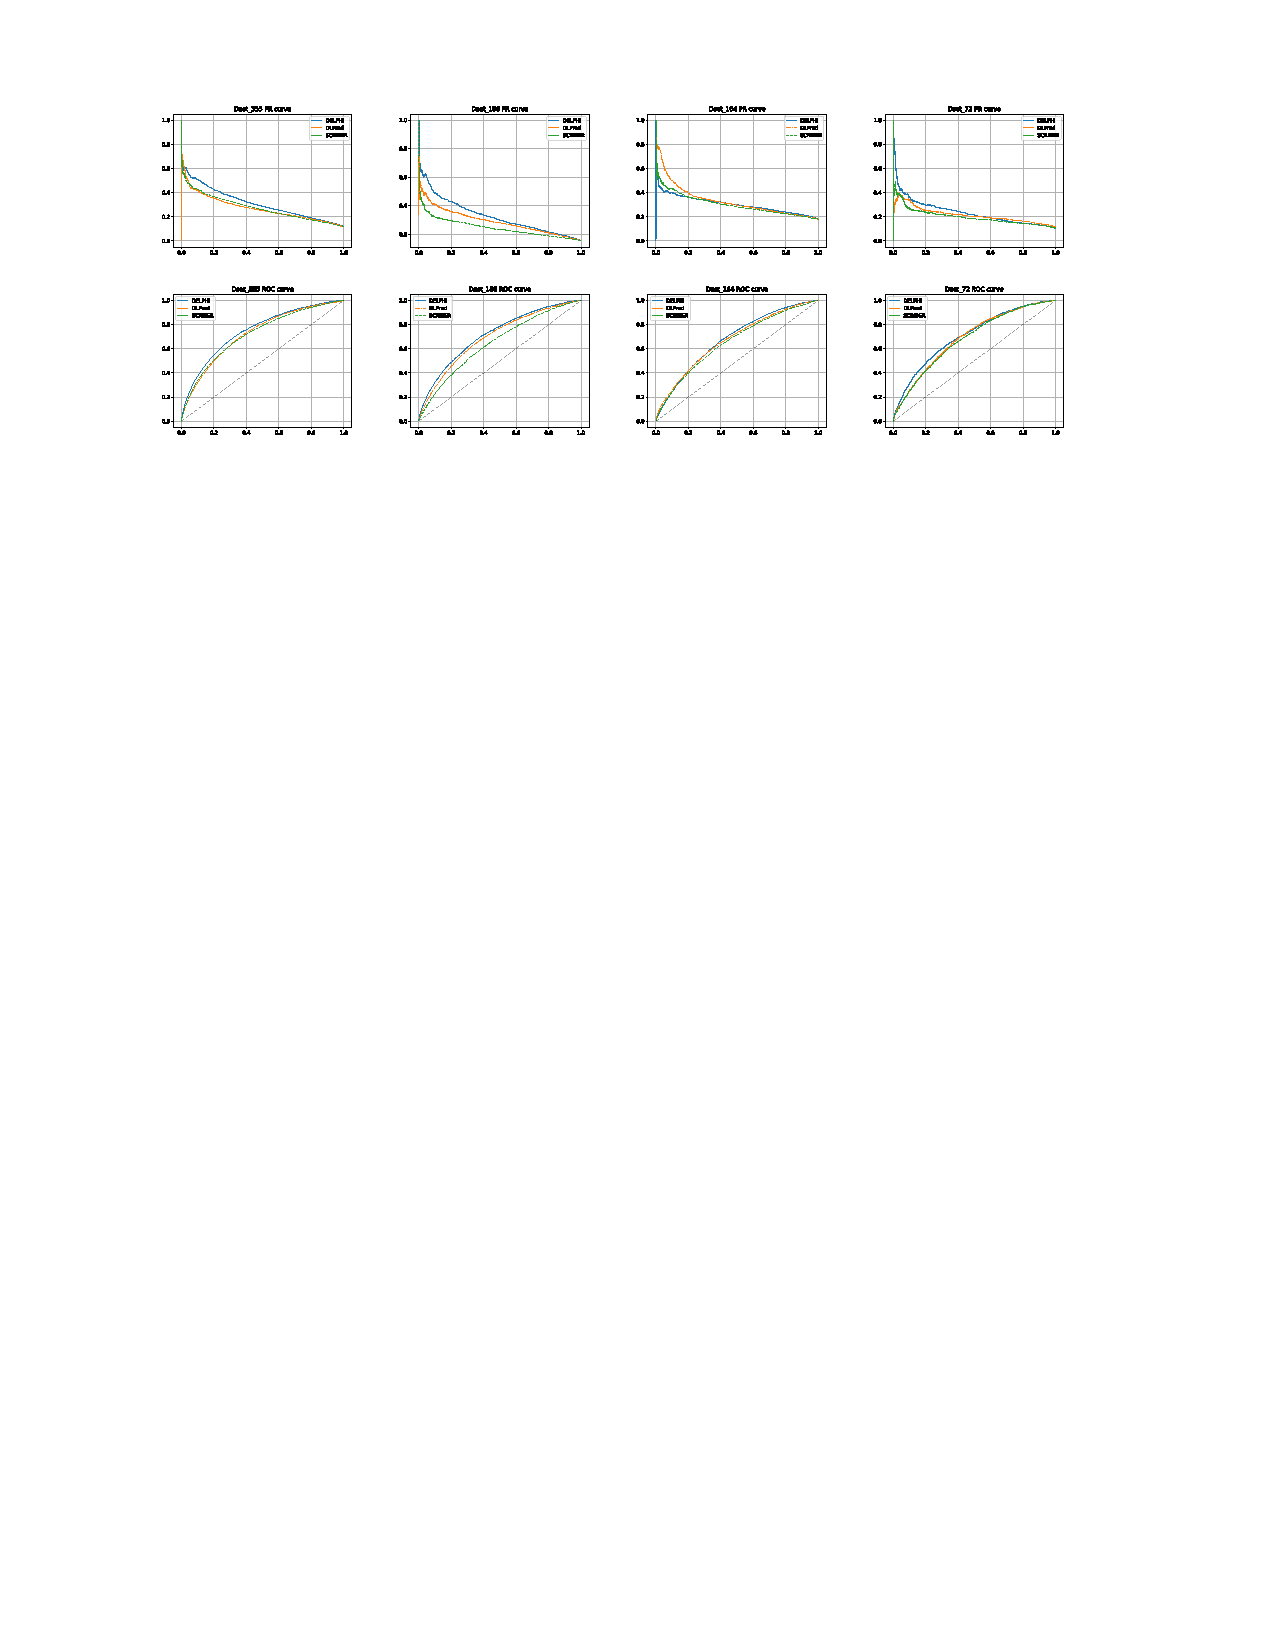
\includegraphics[width=\textwidth]{img/combine_plots.pdf}
%   \caption{The PR curves (top row) and ROC curves (bottom row) for Dset\_355, Dset\_186, Dset\_164, and Dset\_72, from left to right.}
%   \label{fig_ROC_PR}
% \end{figure*}
\section*{Acknowledgements}
We would like to thank Jian Zhang for running SCRIBER on the testing datasets, providing the prediction results of competing methods on Dset\_448 and Dset\_355, and discussing technical details, Buzhong Zhang for running DLPred on Dset\_448, Giancarlo Colmenare for suggestions on tuning the network, Min Zeng for the explanation on DeepPPISP, Alexey Porollo for providing the script for summiting batch jobs to the SPPIDER server, and Tanner Bohn for suggesting using the position information.

\section*{Funding}
The research of L.I. is funded by an NSERC Discovery Grant (R3143A01) and a Research Tools and Instruments Grant (R3143A07). \textcolor{\mySecondColor}{The research of G.B.G. is funded by an NSERC Discovery Grant RGPIN-2020-05733.}

%reference
\bibliographystyle{natbib}

%\bibliographystyle{plain}
%  \clearpage
\bibliography{reference}

\end{document}
